\phantomsection
\subsection*{\centering Noname's ``Blaxploitation''}
\addcontentsline{toc}{subsection}{Noname's ``Blaxploitation''}

\begin{figure}[ht]
    \centering
    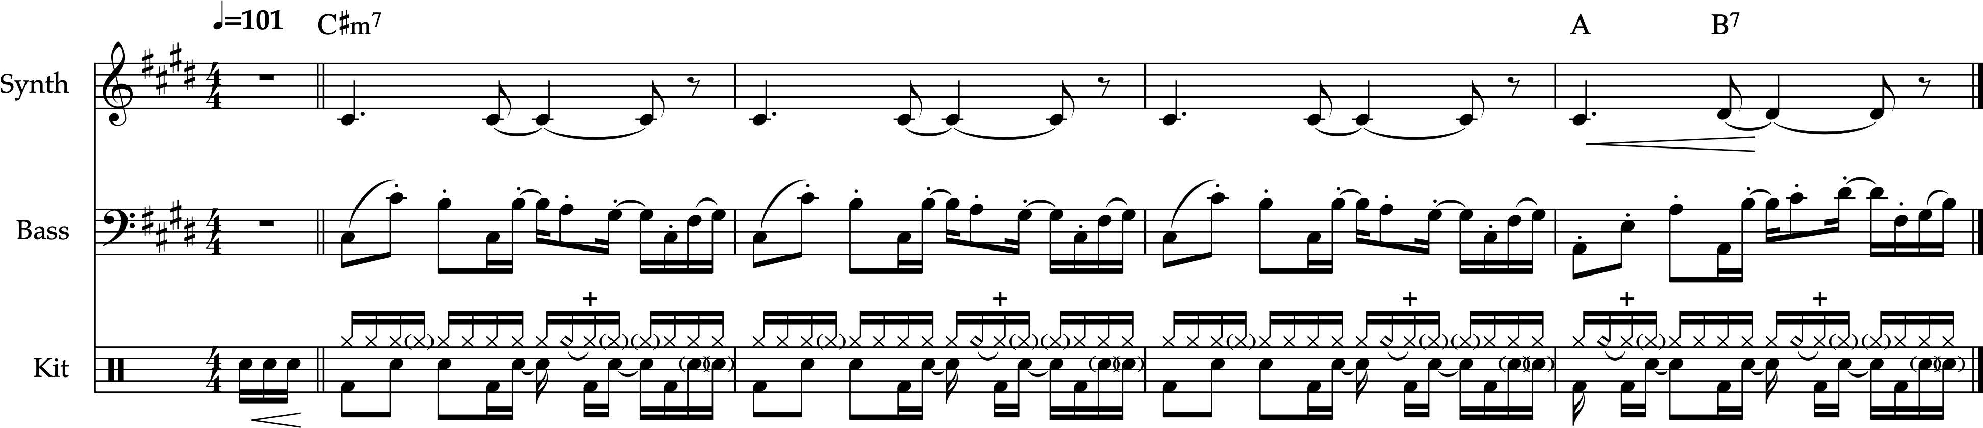
\includegraphics[width=\textwidth]{images/figures/chp 02/006016blaxintro.pdf}
    \caption{Snapshot of the intro to``Blaxploitation,'' 0:06-0:16.}
    \label{fig:blaxploitationintro}
\end{figure}

Phoelix's production on ``Blaxploitation'' centers around an angular, funk bassline that forms a ``functional circuit'' in C-sharp minor.\footnote{\cite{kyleadamsHarmonicSyntacticMotivic2020}.} The drums and bass sound heterogeneously in spite of the relative sparsity of the orchestration due to the frequency of attacks within a short time frame.\footnote{One dimension of the heterogeneous sound ideal is a ``high density of musical events within a relatively short musical time frame''(See \cite{ollywilsonHeterogeneousSoundIdeal1992}, 329.)} Figure~\ref{fig:blaxploitationintro} shows the three primary elements of the basic beat, as well as the sympathetic accentual patterns between the drums and bass.

\begin{table}[ht]
    \centering
    \begin{tabular}{|c|c|c|c|l|}
         \hline
        Section     & Timecode & Duration    & Sample               & Note \\ \hline
        Intro       & 0:00     &             & \textit{Dolemite} I  & \\ \hline
                    & 0:08     & 4 Bars      &                      & \\ \hline
        Verse I     & 0:18     & 12 Bars     &                      & \\ \hline
        \sout{Hook} & 0:46     & 8 Bars      & \textit{Dolemite} II & BGV recomposition \\ \hline
        Verse II    & 1:05     & 12 Bars     &                      & Organ recomposition \\ \hline
        \sout{Hook} & 1:33     & 8 Bars      & \textit{TSWSBTD}     & \\ \hline
        Outro       & 1:52     & 4 Bars      &                      & \\ \hline
    \end{tabular}
    \caption{Condensed roadmap to Noname and Phoelix's ``Blaxploitation.''}
    \label{tab:blaxploitation}
\end{table}

As the track's title suggests, the beat of ``Blaxploitation'' is steeped in the sound of the 1970s, grooving in an allosonic nod to the Motown-inspired soundtracks of the film genre. As shown in Table~\ref{tab:blaxploitation}, the track also autosonically samples dialgoue from two blaxploitation-era films – \textit{Dolemite} (1975) and \textit{The Spook Who Sat by the Door} (1973) – in lieu of hooks. Both of these production decisions instill an air of political consciousness to the track, in keeping with Noname's underground image. 

Joanna Demers notes that the practice of coding the revolutionary politics of Black Americans through a blaxploitation sound is common to hip-hop as an art form. She writes that historically, rappers have ``[monolithically interpreted blaxploitation] films as unified both politically and morally\textellipsis The hip-hop movement neatly compressed [a] more pessimistic view of racial relations under the aegis of Black Power.''\footnote{\cite{joannademersSampling1970sHipHop2003}, 50.} Noname and Phoelix's track participates in this lineage of sounded political consciousness through both autosonic and allosonic techniques.

\clearpage

\begin{sidewaystable}[t]
    \centering
    \small
\begin{tabular}{|c|c|c|c|c|c|c|c|}
     \hline
     Timecode & Noname & Bass & Drums & Synth & Organ & BGVs & Vocal Samples \\ \hline
     0:00-0:07 & & & & & & & \textit{Dolemite} I \\ \hline
     0:08-00:17 & & 3-chord loop & 4-bar funk & C\#-D\# ost & & & \\ \hline
     0:18-0:26 & ``Penny Proud\textellipsis'' & •//• & •//• & & & & \\ \hline
     0:27-0:45 & ``Mmm, yummy\textellipsis'' & ||: 3-chord loop :|| & ||: 4-bar funk :|| & ||: C\#-D\# ost :|| & & & \\ \hline
     0:46-1:04 & & •//• & •//• & •//• & & Countermel. & \textit{Dolemite} II \\ \hline
     1:05-1:23 & ``Anti-political\textellipsis'' & •//• & •//• & •//• & Improv & & \\ \hline
     1:24-1:32 & ``Traded hoodie\textellipsis'' & 3-chord loop & 4-bar funk & C\#-D\# ost & & & \\ \hline
     1:33-1:51 & & ||: 3-chord loop :|| & ||: 4-bar funk :|| & ||: C\#-D\# ost :|| & & Countermel. & \textit{TSWSBTD} \\ \hline
     1:52-2:12 & & 3-chord loop & 4-bar funk & C\#-D\# ost & & & \\ \hline
\end{tabular}
    \caption{Full roadmap to Noname and Phoelix's ``Blaxploitation.''}
    \label{tab:blaxploitationfull}
\end{sidewaystable}